\chapter[Interférence vs. exploitation et dynamique des populations
structurées][Interférence et populations structurées]{Interférence vs.
exploitation et dynamique des populations structurées}
\label{chap:amnat}

\vspace{2cm}
\begin{Spacing}{1}
\texttt{
Le Bourlot, Vincent, Thomas Tully and David Claessen, "Interference versus
Exploitative Competition in the regulation of Size-Structured Populations"\\
under review at The American Naturalist
}
\end{Spacing}
\vspace{2cm}


\lettrine[lines=3]{D}{ans le chapitre} précédent, nous avons pu voir le rôle
prépondérant que jouent les individus de grande taille dans la régulation des
populations de collembole \textit{Folsomia candida} élevés en laboratoire. Les
individus de grande taille impactent fortement la population par l'intermédiaire
des interactions entre individus et de la compétition pour les ressources. La
compétition est un des facteurs principaux dans la régulation de la dynamique
des populations et des communautés. Son effet peut être soit direct entre
plusieurs individus via la compétition par interférence, ou par l'intermédiaire
de la ressource dans la compétition par exploitation.

L'impact de la compétition par exploitation sur la dynamique des populations a
déjà été largement étudié, tant d'un point de vue empirique que théorique, mais
les effets de la compétition par interférence restent quant à eux mal compris.
Nous avons déjà montré empiriquement le rôle de l'interférence dans la
régulation de la dynamique des populations structurées, mais à ce jour, il
n'existe pas encore de cadre théorique aux effets de la compétition par
interférence sur les populations structurées.

Nous étudions dans ce chapitre les effets de différents niveaux de compétition
intra-spécifique par interférence sur la dynamique d'une population structurée
en taille. Nous basons notre étude sur un modèle ressource -- consommateur
physiologiquement structuré \autocites[modèle de ][]{kooijman1984a} prenant
en compte des interactions directes entre les individus, autorisant ainsi un
gradient depuis une compétition purement par exploitation à une compétition
totalement dominée par l'interférence. Nous paramétrons notre modèle en
utilisant les données issues des suivis expérimentaux de populations de
collemboles \textit{Folsomia candida}.

Notre modèle prédit une variété de dynamiques possibles suivant le niveau de
compétition par interférence imposé. A un faible niveau d'interférence, notre
modèle se comporte de manière similaire au modèle classique de Kooijman et Metz.
Un niveau plus fort d'interférence agit comme une force stabilisatrice sur les
cycles de générations causés par les juvéniles. A niveau intermédiaire, des
géants émergent dans la populations et commencent à la dominer. Enfin, à un
niveau très élevé d'interférence, un nouveau type de cycle apparaît que l'on
appelle cycles causés par l'interférence. Nos résultats théorique permettent
d'apporter un nouvel éclairage dans l'interprétation des dynamiques de la
structure en taille des populations de collemboles élevées au laboratoire.

\section{Éléments de méthodologie}


\subsection{Définition du modèle}

\subsubsection{Paramètres du modèle}

Notre modèle repose sur celui développé par
\textcites[KM-model][]{kooijman1984a} et \textcites{de-roos1992a}. Ce modèle
est un modèle mécaniste qui défini les processus au niveau individuel et laisse
la dynamique émerger au niveau de la population. Les paramètres du
modèle sont tirés des suivis expérimentaux des populations de collembole
présentés dans le Chapitre précédent. Les paramètres sont rappelés dans la Table
\ref{tab:ANparam}. Les données expérimentales permettant de justifier ces
données sont présentées dans les Supplementary Materials \ref{subsec:SupMat1} de
l'Annexe \ref{An:AmNat}. 

\begin{table}
\caption{\label{tab:ANparam}Variables et paramètres pour \textit{Folsomia
candida}}
\begin{tabular}{cccl}
\hline
\hline 
 & & &\\
 Objects and  & Default values & Units & Description\\ 
symbols & & &\\
\hline
	$i$-state variable & & & \\ 
	$l$ &   & mm & Individual length \\ 
	Parameters & & & \\ 
	$l_{b}$ & 0.25 & mm & Length at birth \\ 
	$l_{j}$ & 0.6 & mm & Length at maturity \\ 
	$l_{m}$ & 3.0 & mm & Length at infinite\\
	& & &  resources \\ 
	$\gamma$ & 0.015 & d$^{-1}$ & Van Bertalanffy growth rate \\ 
	$\eta_{H}$ & 1000 & individuals & Half saturation constant \\ 
	$\mu$ & 0.0065 & d$^{-1}$ & Background mortality \\ 
	$r_{m}$ & 3.0 & d$^{-1}$mm$^{-2}$ & Reproduction rate \\ 
	$\kappa$ & 0.7 & -- & Fraction of energy \\
	  &   &   & intake allocated \\
	  &   &   & to reproduction \\ 
	  $I$ & 0 & -- & Level of interference\\
\hline 
\end{tabular} 
\end{table}

\subsubsection{Densité dépendance}

L'objectif de ce modèle est de prendre en compte les
processus d'interférence dans les mécanismes de densité dépendance qui régulent la population. Nous avons
défini l'état physiologique d'un individu par sa longueur corporelle $l$. Cette
longueur varie de la taille à la naissance $l_b$ à la taille maximum atteignable
sans aucune compétition $l_m$. Nous décrivons les interations individuelles au
travers de la fonction $A(t,l)$. Cette fonction que l'on appelle fonction
``d'accès à la ressource'' dépend de la densité de la population telle qu'elle
est resentie par un individu, en fonction de sa taille. Cette densité resentie,
notée $\eta (t,l)$, repose sur le fait qu'un individu de petite taille est plus
impacté par la présence d'un individu de grande taille que l'inverse. Les
paramètres de la fonction $A$ nous permettent alors d'ajuster le niveau de
compétition par interférence dans la population. Cette fonction est définie
comme suit, avec $\eta _H$ un coefficient de demi-saturation:

\begin{equation}
\label{eq_an1}
A(t,l)=1-\frac{\eta(t,l)}{\eta_H+\eta(t,l) }  
\end{equation}

La densité resentie $\eta$ est définie pour un individu de taille $l$, au temps
$t$, par:

\begin{equation}
\label{eq_an2}
\eta(t,l)=\int_{l_b}^{l_m} \! C(l,\lambda)\cdot n(t,\lambda)\cdot\lambda^2\, \mathrm{d}\lambda
\end{equation}

La densité de la population resentie par un individu dépend donc de la structure
effective de la population, et d'une fonction de compétition $C(\lambda ,l)$.
Cette fonction de compétition représente la supériorité d'un individu de taille
$\lambda$ sur un individu de taille $l$ en fonction de la différence de taille
entre les deux:

\begin{equation}
\label{eq_an3}
C(l,\lambda) = \mathrm{max}\left[ 0.01,\, 1+I\cdot(\lambda-l) \right]
\end{equation}

où $I$ est le paramètre d'interférence qui permet de régler le niveau de
compétition par interférence dans la population. $I=0$ conduira à une population
régulée uniquement par de la compétition par exploitation. 

\subsubsection{règle du $\kappa$ et taux individuels}

Outre les interactions entre individus, le modèle se base sur les règles
d'allocation dynamiques du budget énergétique \autocites{kooijman2000a}. Une fois la règle fixée, on peut en
dériver les taux vitaux individuels. 

\begin{figure}[!ht]
\begin{center}
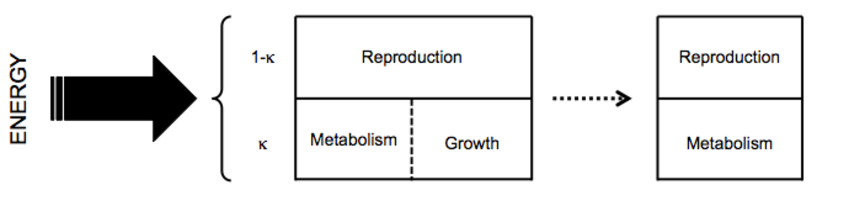
\includegraphics[width=0.95\textwidth]{1_CorpsDeThese/Resumes/Fig/AN01}
\caption[\lofimage{1_CorpsDeThese/Resumes/Fig/AN01}Règle du
$\kappa$$]{Schéma de la règle du $\kappa$ et de ses implication}
\label{fig:AN1}
\end{center}
\end{figure}

Nous nous basons sur la règle d'allocation appelée règle du
$\kappa$ ($\kappa$-rule), schématisée par la Figure \ref{fig:AN1}. Cette règle
suppose qu'une proportion $\kappa$ de l'énergie acquise par un individu est
allouée à la maintenance (métabolisme) et à la croissance, le reste ($1-\kappa$)
étant attribué à la reproduction. Cela implique automatiquement qu'un individu à sa
taille maximum continue de se reproduire, ce qui n'est pas toujours le cas pour
d'autres règles d'allocation de l'énergie (voir Annexe \ref{An:AmNat},
Supplementary Materials \ref{subsec:SupMat4}). Si l'énergie acquise n'est pas
suffisante pour couvrir l'intégralité du métabolisme, l'individu meure. 

En supposant que l'acquisition de la ressource est proportionnelle à $l^2$
et que le métabolisme est proportionnel à $l^3$, cette règle d'allocation de
l'énergie nous permet de définir les taux vitaux individuels tels que décrit
dans la Table \ref{tab:ANeq}. Le détail de la dérivation des équations du modèle
est disponible dans les Supplémentary Materials \ref{subsubsec:SupMat21} de
l'Annexe \ref{An:AmNat}. 

\begin{table}
\centering
\caption{\label{tab:ANEq} Equations du modèle d'après la règle du $\kappa$.}
\begin{tabular}{cl}
\hline 
\hline
&\\
Equation & Description \\
\hline
	$\displaystyle{A(t,l)=1-\frac{\eta(t,l)}{\eta_{H}+\eta(t,l)}}$ & Access to the
	resource\\
	&\\
	$\displaystyle{\eta (t,l) = \int\limits_{l_b}^{l_m} C(l,\lambda)\cdot
	n(t,\lambda)\cdot \lambda^2\,\text{d}\lambda}$ & Experienced population
	density\\
	&\\
	$\displaystyle{C(l,\lambda) = \text{max}[0.01,\, 1+I\cdot(\lambda-l)]}$ &
	Competition function \\
	&\\
	$\displaystyle{g(t,l) = \gamma\cdot(l_m \cdot A(t,l)-l)}$ & Growth rate\\
	&\\
	$\displaystyle{b(t,l) = r_m \cdot A(t,l)\cdot l^2}$ & Birth rate if $l\geq
	l_j$\\
	&\\
	&\\
	$\displaystyle{\frac{\partial n(t,l)}{\partial t}+ \frac{\partial
	g(t,l)\cdot n(t,l)}{\partial l} = -\mu \cdot n(t,l) }$ & Population level
	equation\\
	&\\
	$\displaystyle{g(t,l_b)\cdot n(t,l_b) = \int\limits_{l_b}^{l_m} b(t,l)\cdot
	n(t,l) \, \text{d}l}$ & Boundary conditions \\
\hline 
\end{tabular} 
\end{table}

\subsubsection{Minimum vital d'accès au ressources}
Nous définissons le minimum vital d'accès aux ressources comme la quantité $A^*$
telle que la croissance individuelle est nulle. Bien que dépendante de $l$,
cette quantité:
\begin{equation}
\label{eq_an4}
A^*(l) = \frac{l}{l_m}
\end{equation}
est analogue au $R^*$ de Tilman dans le sens où elle définit des conditions
minimums permettant la croissance des individus. 

\subsubsection{Intégration au niveau population}

Au niveau de la population, le nombre d'individus au temps $t$ est donné par
\begin{equation}
\label{eq_an5}
\int_{l_b}^{l_m}\!n(t,l)\,\mathrm{d}l
\end{equation}
où $n(t,l)$ est le nombre d'individus de taille $l$ au temps $t$. La dynamique
de la population est alors donnée par les équations et conditions initiales
suivantes \autocites{kooijman1984a,de-roos1997a}:
\begin{align}
\label{eq_an6}
\frac{\partial n(t,l)}{\partial t}+\frac{\partial g(t,l) \cdot n(t,l)}{\partial l}=-\mu \cdot n(t,l) \\
g(t,l_b) \cdot n(t,l_b)= \int_{l_b} ^{l_m} \! b(t,l)\cdot n(t,l)\, \mathrm(d)l
\\ n(0,l)=\Psi(l)
\end{align}

\subsection{Analyse de bifurcation}

Afin d'étudier le rôle de l'interférence dans les dynamiques produites par notre
modèle, nous avons réalisé une analyse de bifurcation sur le paramètre $I$ du
modèle. Bien que cette analyse ne soit pas une analyse de continuation à
proprement parler, elle nous permet d'identifier les intervalles de paramètre
correspondant à différents types de dynamiques. 

Le principe de cette analyse est comme suit: (i) une première simulation est
exécutée avec la valeur initial du paramètre dit de bifurcation (ici $I$)
jusqu'à ce que la population ait quitté le régime transitoire; (ii) l'état final
de la population (soit sa distribution à la fin de la simulation) est utilisé
comme état initial d'une nouvelle simulation; (iii) le paramètre d'interférence
est incrémenté; et (iv) le processus est répété jusqu'à exploration de
l'ensemble de l'intervalle voulu. Notons que cette analyse peut également être
réalisée avec des valeurs décroissantes du paramètre de bifurcation, ce qui peut
permettre d'identifier des zones de bistabilité. 

Dans un premier temps, cette analyse a été réalisée pour une valeur fixe des
paramètres excepté le paramètre de bifurcation $I$. Puis, sachant que la
mortalité a un fort effet sur la dynamique de ce type de modèle, cette analyse
a été faite pour des valeurs successives de mortalité avec le paramètre $I$
comme paramètre de bifurcation, et pour des valeurs successives d'interférence
avec le paramètre de mortalité $\mu$ comme paramètre de bifurcation. Ainsi,
l'ensemble de l'espace $(I,\mu)$ a été quadrié pour des valeurs de $I$ de 0 à 3
et des valeurs de $\mu$ de 0.001 à 0.02

\section{Résultats}

Nous nous intéressons dans un premier temps à l'effet du niveau de compétition
par interférence pour une valeur assez faible de mortalité ($\mu = 0.0065$,
Figure \ref{fig:AN2}). 

\begin{figure}[!ht]
\begin{center}
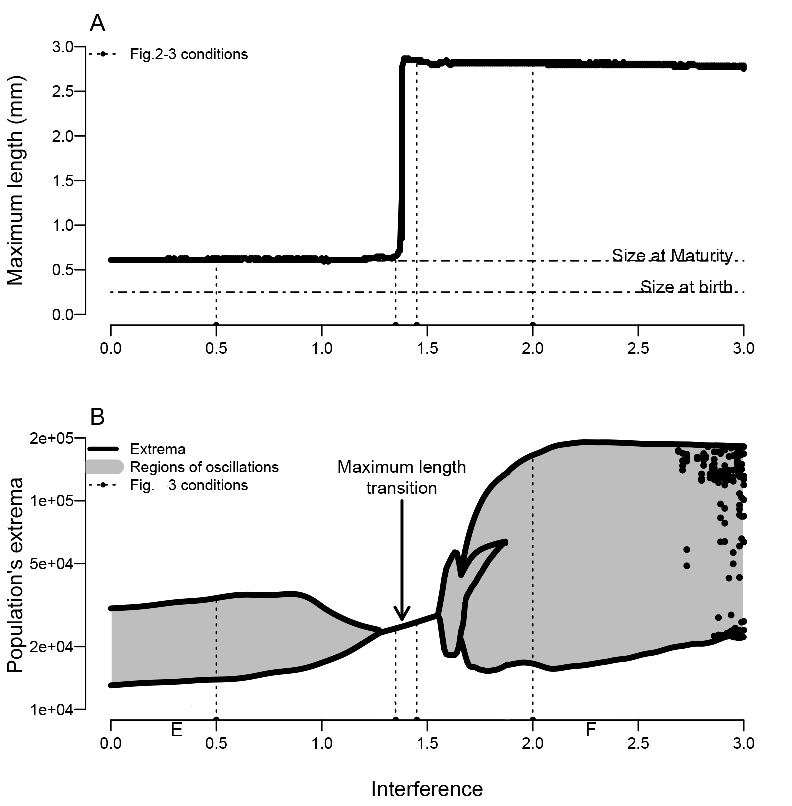
\includegraphics[width=0.95\textwidth]{1_CorpsDeThese/Resumes/Fig/AN02}
\caption[\lofimage{1_CorpsDeThese/Resumes/Fig/AN02}Bifurcation sur le
niveau d'interférence]{Taille maximum atteinte dans la population (A) et extrema
de la population (B, nombre d'individus) en fonction du niveau de compétition par interférence $I$ pour une
valeur constante de mortalité ($\mu = 0.0065$). Les lignes pointillées
représentent les valeur d'interférence des simulations présentées en Figure
\ref{fig:AN3}. Les zones grisées marquent les zones ou la population est
cyclique. La flèche marque la transition de taille maximum atteinte.}
\label{fig:AN2}
\end{center}
\end{figure}

On constate dans un premier temps qu'un niveau suffisamment élevé de compétition
par interférence ($I=1.4$) provoque une transition dans la taille maximum
atteinte par les individus (Figure \ref{fig:AN2}A). Lorsque le niveau
d'interférence est plus faible que cette valeur, la taille maximum atteint ($l=0.63mm$) reste proche de la taille à
maturité ($l_j=0.6mm$). Au delà de la valeur critique, la taille atteinte
($l=2.85mm$) se rapproche fortement de la taille maximum atteignable
($l_m=3mm$). 

De plus, la Figure \ref{fig:AN2}B montre trois régions distinctes: (i) à faible
interférence, la population est cyclique; (ii) pour un niveau intermédiaire de
compétition par interférence, la population est stable; et (iii) pour une forte
interférence, la population cycle autour d'un nouveau type de cycles de plus
grande amplitude que les précédents. 

\subsection{Des cycles dirigés par les juvéniles}

Les modèles PSP classiques prédisent qu'à faible mortalité, la différence de
capacité de compétition entre les juvéniles et les adultes conduit à des cycles
de génération dirigés par les juvéniles \autocites{de-roos1992a,de-roos1997a}.
La Figure \ref{fig:AN3}abc montre la dynamique de la population pour un faible
niveau d'interférence ($I=0.5$). On observe sur le diagramme structure-temps (a)
que la dynamique cyclique correspond à des vagues successives de recrutement de
juvéniles avec des adultes ne dépassant que très peu la taille à maturité. Cette
dynamique est caractéristique des cycles de génération dirigés par les juvéniles
\autocites{de-roos1992a,de-roos2003a}.

\afterpage{%
    \clearpage% flush all other floats
    \ifodd\value{page}
    %\else% uncomment this else to get odd/even instead of even/odd
        \expandafter\afterpage% put it on the next page if this one is odd
    \fi
    {%
    \begin{figure}[p]
        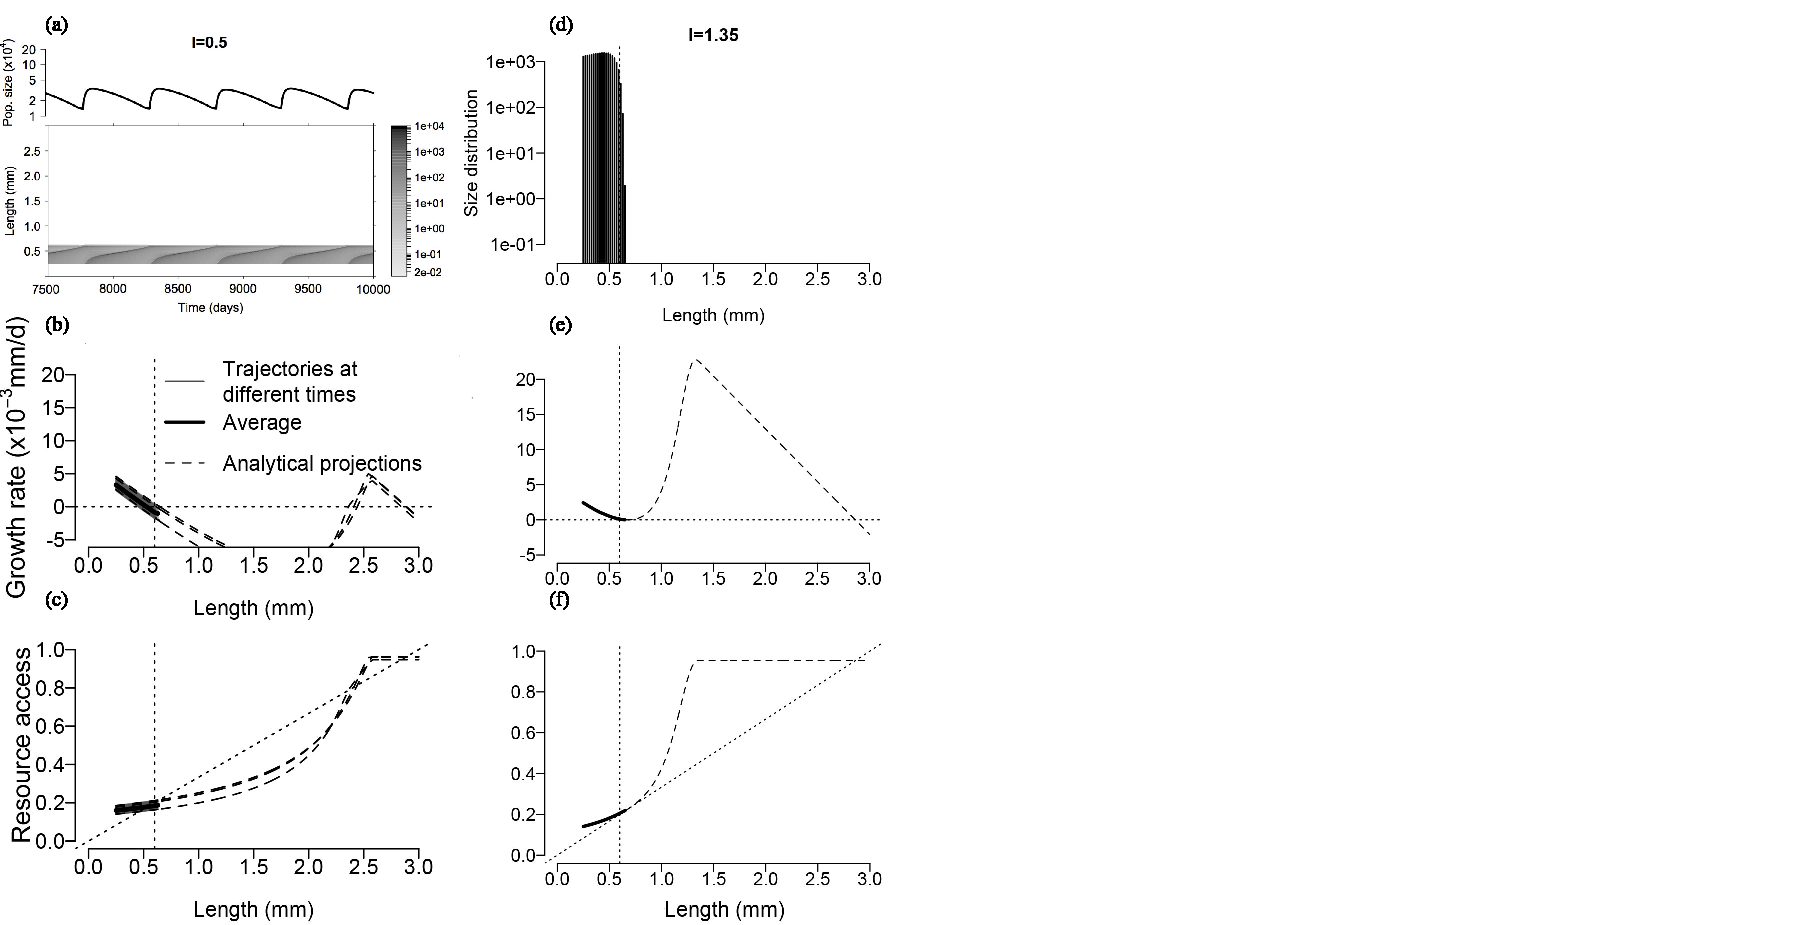
\includegraphics[width=\textwidth]{1_CorpsDeThese/Resumes/Fig/AN03}
        \caption{Exemples de dynamiques pour quatre valeurs d'interférence: 0.5,
1.5, 1.45 et 2.0. La première ligne de panels (a,d,g,j) montre soit la
dynamique de la structure à l'aide d'un diagramme structure-temps (a,j), soit la
distribution de la taille si elle est stable dans le temps (d,g). La seconde
ligne (b,e,h,k) représente le taux de croissance en fonction de la longueur
corporelle\ldots}\label{fig:AN3}
    \end{figure}
    \clearpage
    \begin{figure}[p]
		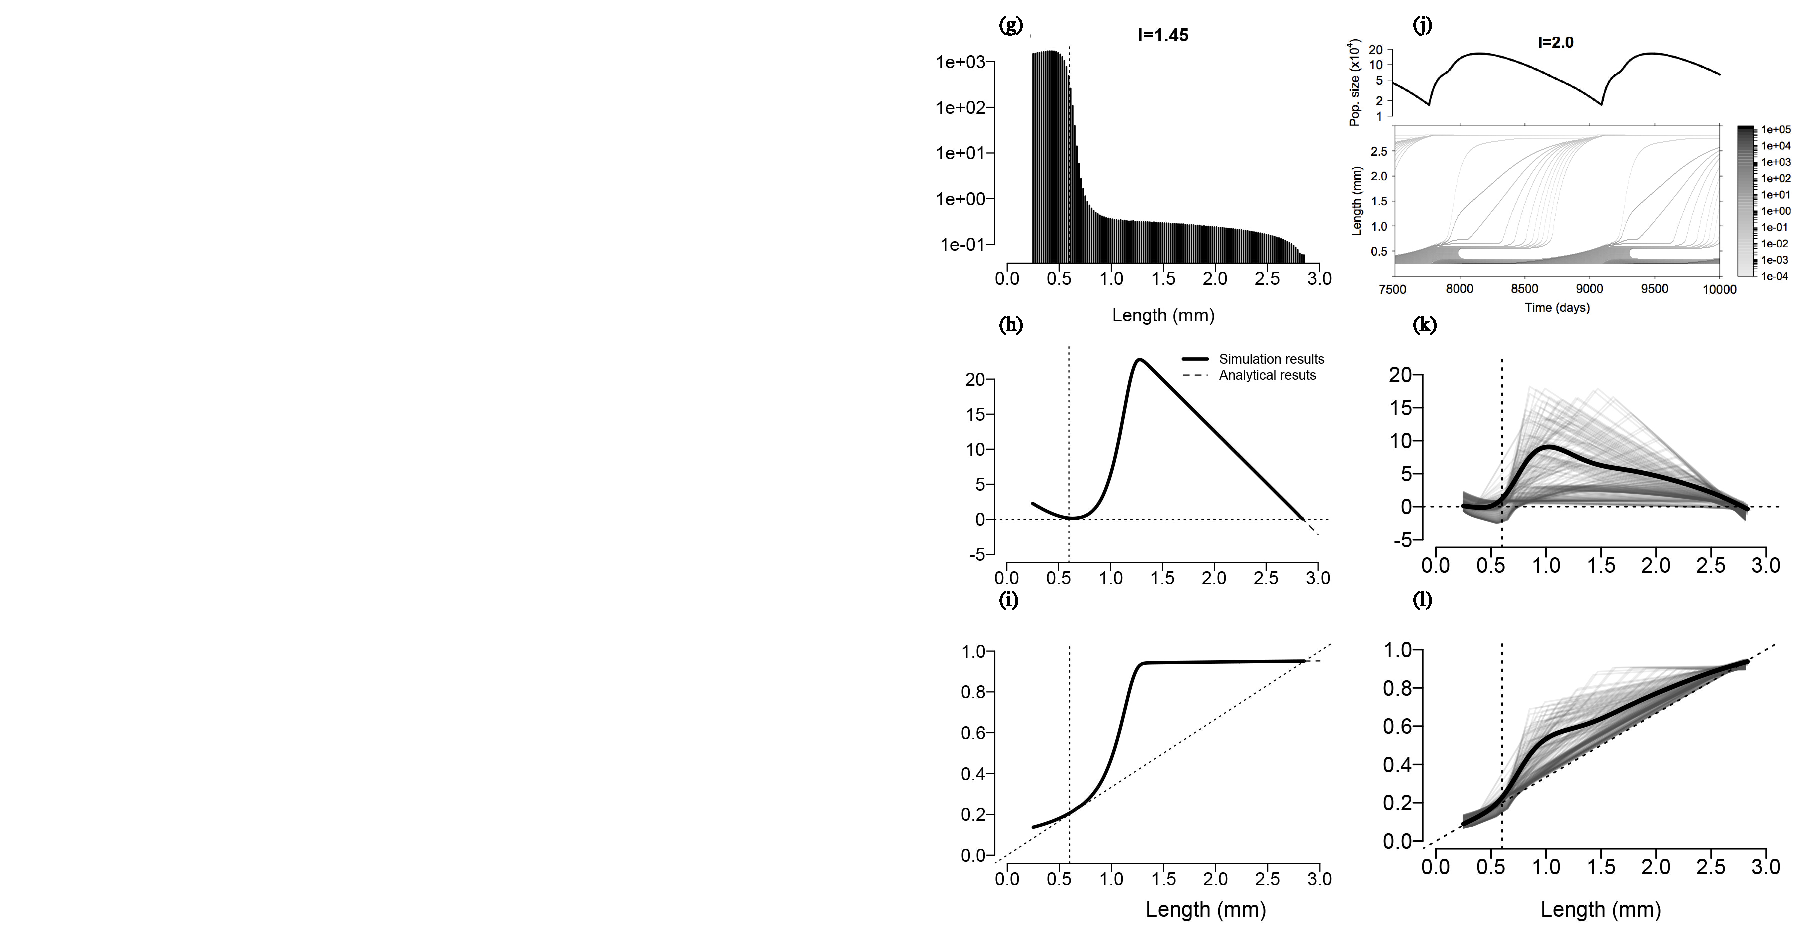
\includegraphics[width=\textwidth]{1_CorpsDeThese/Resumes/Fig/AN04}
        \caption*{\ldots Lorsque la dynamique est cyclique, plusieurs
        trajectoires sont présentées, ainsi que leur moyenne en trait épais.La ligne pointillée
horizontale est le 0, la ligne verticale marque la taille à maturité. Enfin, la
dernière ligne de panels (c,f,i,l) présente l'accès à la ressource. La ligne
verticale marque la taille à maturité, la ligne oblique marque l'accès minimum
requis $A^*$. Pour le taux de croissance et l'accès aux ressources, les lignes
tiretées représentent les projections analytique des fonctions tracées.}
    \end{figure}
    \clearpage
    }%
}

Les Figures \ref{fig:AN3}b et c montrent le taux de croissance et l'accès au
ressources pour cette dynamique. Le taux de croissance décroît
quasi-linéairement avec la taille, de façon très similaire au modèle classique
sans interférence. L'accès aux ressources est très légèrement croissant mais
devient rapidement inférieur à $A^*$ pour tous les individus après la maturité. 

\subsection{Un équilibre stable avec des petits ou des géants}

Pour des valeurs intermédiaires de compétition par interférence, l'avantage
que les grands individus retirent de l'interférence contrebalance la compétition
par exploitation imposée par les juvéniles. Ceci vient contrer les mécanismes
de déséquilibre compétitif à l'origine des cycles de génération, et tend à
stabiliser la population (Figure \ref{fig:AN3}d-j).

Pour une valeur d'interférence sous le seuil critique de $I=1.4$, la dynamique
se stabilise autour d'une distribution étroite de la taille corporelle (Figure
\ref{fig:AN3}d). Le taux de croissance et l'accès à la ressource ont tendance à
se courber vers le haut pour les plus grands individus, mais la courbure n'est
pas suffisante pour permettre à l'accès au ressources de rester au dessus de
$A^*$, et les individus s'arrêtent de grandir rapidement après la maturation (Figure
\ref{fig:AN3}ef).

Au delà de ce seuil critique, la courbure est suffisante pour que l'accès aux
ressources soit toujours supérieur à $A^*$ et le taux de croissance soit
toujours positif (Figure \ref{fig:AN3}hi). Après un ralentissement de leur
croissance proche de la maturité (``goulet d'étranglement de la croissance''), les individus peuvent
reprendre une croissance rapide jusqu'à des tailles très élevées. La
distribution de la taille dans la population est alors très asymétrique vers les
juvéniles, mais reste continue jusqu'à des tailles proches de la taille maximum
possible $l_m$ (Figure \ref{fig:AN3}g).
